\documentclass[11pt]{article}
\usepackage[spanish]{babel}
\usepackage{amsmath}
\usepackage{amssymb}
\usepackage{graphicx}
\graphicspath{ {./images/}, {~/Apunte/images/} }
\usepackage[utf8]{inputenc}
\usepackage[T1]{fontenc}
\usepackage[margin=1in]{geometry}
\usepackage{fancyhdr}
\usepackage{hyperref}

\hypersetup{
    pdftitle={Reporte Post-Laboratorio 03: Presentaciones en Beamer},
    pdfauthor={Felipe Colli Olea},
    colorlinks=true,
    linkcolor=black,
    urlcolor=cyan
}

\pagestyle{fancy}
\fancyhf{}
\fancyfoot[C]{\footnotesize Felipe Colli, Todos los Derechos Reservados}
\fancyfoot[R]{\thepage}
\renewcommand{\headrulewidth}{0pt}

\title{Reporte Post-Laboratorio 03: \\ Diseño de Presentaciones con la clase \texttt{beamer}}
\author{Felipe Colli Olea}
\date{\today}

\begin{document}

\maketitle
\thispagestyle{fancy}

\section{Introducción}
El presente reporte documenta el trabajo realizado en el Laboratorio 03, cuyo objetivo principal fue la transición desde la redacción de documentos continuos (clase \texttt{article}) hacia la creación de material de apoyo visual para exposiciones orales utilizando la clase \texttt{beamer} de \LaTeX. Para poner en práctica estos conceptos, se desarrolló una presentación sobre las Leyes de Newton y la biografía del físico.

\section{Cambio de Lógica: De Artículo a Presentación}
Como se analizó en el material teórico del curso, aprender \texttt{beamer} no implica empezar desde cero, sino que requiere un \textbf{cambio de lógica visual}. Mientras que un artículo está pensado para la lectura continua a través de secciones y párrafos, una presentación organiza la información para marcar el ritmo de una exposición oral.

Estructuralmente, el esqueleto del documento cambia: el contenido ya no fluye libremente, sino que debe encapsularse dentro de entornos \texttt{\textbackslash begin\{frame\}}.

\section{Análisis de la Implementación (Leyes de Newton)}
Durante el desarrollo del laboratorio, se implementaron diversas herramientas de maquetación visual que \texttt{beamer} ofrece para organizar la información:

\begin{figure}[h]
	\centering
	% REEMPLAZA ESTO CON UN PANTALLAZO DE TU CÓDIGO EN NEOVIM O EL PDF COMPILADO DE LA DIAPOSITIVA DE LA BIOGRAFÍA
	
\includegraphics[width=0.8\textwidth]{nvim.png}
	\caption{Uso del entorno \texttt{columns} para la biografía de Newton.}
	\label{fig:columnas}
\end{figure}

\subsection{Layout Libre: Columnas y Bloques}
Para evitar la monotonía del texto plano y aprovechar el espacio de la diapositiva, se utilizaron dos recursos clave:
\begin{itemize}
	\item \textbf{Entorno \texttt{columns}:} Implementado en la diapositiva de la biografía de Newton (ver Figura \ref{fig:columnas}), permitió dividir el layout en una columna izquierda (60\% del ancho) para las viñetas explicativas, y una columna derecha (40\%) para insertar de forma ordenada la imagen del físico usando \texttt{\textbackslash includegraphics}.
	\item \textbf{Bloques semánticos (\texttt{block}):} Utilizados en la diapositiva de la Segunda Ley de Newton, permitieron jerarquizar la información separando visualmente la "Descripción", la "Ecuación" y el "Ejemplo en la vida cotidiana".
\end{itemize}

\begin{figure}[h]
	\centering
	% REEMPLAZA ESTO CON UN PANTALLAZO DE TU CÓDIGO MOSTRANDO LAS ECUACIONES O EL BIBTEX
	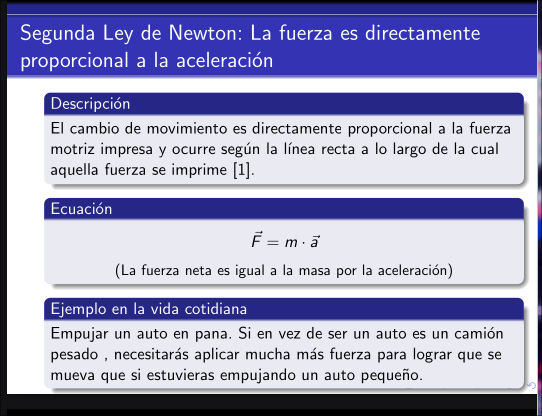
\includegraphics[width=0.8\textwidth]{forms.png}
	\caption{Implementación de bloques y ecuaciones en el entorno frame.}
	\label{fig:ecuaciones}
\end{figure}

\subsection{Continuidad de Fórmulas y Bibliografía}
Un aspecto destacable de este entorno de trabajo es que la potencia matemática de \LaTeX{} se mantiene intacta. Como se observa en la Figura \ref{fig:ecuaciones}, el uso de fórmulas matemáticas en modo destacado (ej. $\vec{F} = m \cdot \vec{a}$ y $\sum \vec{F} = 0$) funcionó exactamente igual que en un documento normal. Asimismo, el sistema de referencias mediante BibTeX (\texttt{\textbackslash cite}) permitió generar la bibliografía en el último frame sin requerir configuraciones ajenas a las convencionales.

\section{Conclusión}
El trabajo con \texttt{beamer} demuestra que, teniendo una base sólida en el lenguaje \LaTeX, la creación de presentaciones de alta calidad tipográfica es un proceso sumamente directo. El uso de temas (como \textit{Darmstadt}) y herramientas de distribución visual garantiza un resultado mucho más estable y profesional que el de los softwares ofimáticos tradicionales.

\end{document}
